\documentclass{article}
% Shared style for the LUMEN manuscript diagrams (\input by every fig_*.tex; class: article).
% Uses only fonts and packages of a basic TeX installation (Computer Modern Sans), so compiling
% never triggers a package download. Each figure is wrapped in the lumenfig environment, which
% ships the picture out as a single page cropped to the drawing plus a 3 pt margin.
\usepackage{amsmath,amssymb}
\renewcommand{\familydefault}{\sfdefault}
\usepackage{tikz}
\usetikzlibrary{positioning,arrows.meta,fit,backgrounds,calc,shapes.geometric,decorations.pathreplacing}
\pagestyle{empty}

\newsavebox{\lumenfigbox}
\newenvironment{lumenfig}%
  {\begin{lrbox}{\lumenfigbox}}%
  {\end{lrbox}%
   \pdfpagewidth=\dimexpr\wd\lumenfigbox+6pt\relax
   \pdfpageheight=\dimexpr\ht\lumenfigbox+\dp\lumenfigbox+6pt\relax
   \hoffset=-1in\voffset=-1in
   \shipout\vbox{\kern3pt\hbox{\kern3pt\usebox{\lumenfigbox}}}}

% palette: physics (blue), learning (green), data (amber), reporting (violet), neutral ink
\definecolor{ink}{HTML}{1F2933}
\definecolor{muted}{HTML}{52606D}
\definecolor{rule}{HTML}{CBD2D9}
\definecolor{phyE}{HTML}{3B6EA8}\definecolor{phyF}{HTML}{E8F1FB}
\definecolor{lrnE}{HTML}{3C8C5A}\definecolor{lrnF}{HTML}{EAF6EE}
\definecolor{datE}{HTML}{B7791F}\definecolor{datF}{HTML}{FDF3E4}
\definecolor{outE}{HTML}{6B4FA0}\definecolor{outF}{HTML}{F3EEFB}
\definecolor{grey}{HTML}{9AA5B1}

\tikzset{
  >={Stealth[length=2.4mm,width=1.8mm]},
  every node/.style={font=\footnotesize, text=ink},
  box/.style={draw, rounded corners=2.5pt, line width=0.7pt, align=center, inner sep=4pt,
    execute at begin node={\hyphenpenalty=10000\exhyphenpenalty=10000}},
  phy/.style={box, draw=phyE, fill=phyF},
  lrn/.style={box, draw=lrnE, fill=lrnF},
  dat/.style={box, draw=datE, fill=datF},
  rep/.style={box, draw=outE, fill=outF},
  neutral/.style={box, draw=grey, fill=white},
  flow/.style={->, line width=0.8pt, draw=ink},
  soft/.style={->, line width=0.7pt, draw=muted, dashed},
  title/.style={font=\footnotesize\bfseries},
  note/.style={font=\scriptsize, text=muted, align=center},
  stage/.style={draw=rule, rounded corners=4pt, line width=0.6pt, dashed, inner sep=6pt},
  stagelabel/.style={font=\scriptsize\bfseries, text=muted, anchor=south west, inner sep=1pt},
}

\begin{document}
\begin{lumenfig}
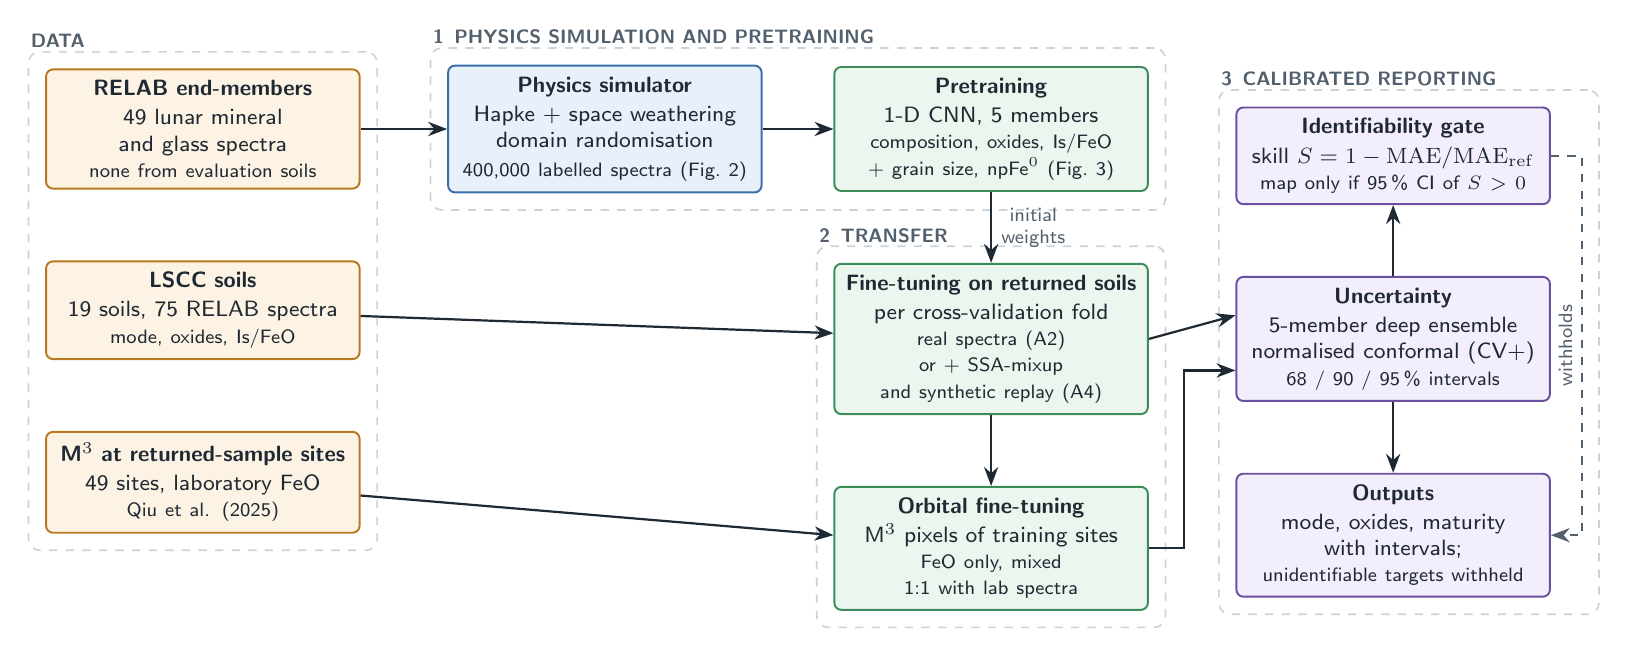
\begin{tikzpicture}[node distance=5mm and 7mm]

% ---- data sources (left column)
\node[dat, text width=37mm] (relab) {\textbf{RELAB end-members}\\[1pt]49 lunar mineral and glass spectra\\{\scriptsize none from evaluation soils}};
\node[dat, text width=37mm, below=9mm of relab] (lscc) {\textbf{LSCC soils}\\[1pt]19 soils, 75 RELAB spectra\\{\scriptsize mode, oxides, Is/FeO}};
\node[dat, text width=37mm, below=9mm of lscc] (m3) {\textbf{M$^3$ at returned-sample sites}\\[1pt]49 sites, laboratory FeO\\{\scriptsize Qiu et al. (2025)}};

% ---- stage 1: physics
\node[phy, text width=37mm, right=11mm of relab] (sim) {\textbf{Physics simulator}\\[1pt]Hapke + space weathering\\domain randomisation\\[1pt]{\scriptsize 400{,}000 labelled spectra (Fig.~2)}};
\node[lrn, text width=37mm, right=9mm of sim] (pre) {\textbf{Pretraining}\\[1pt]1-D CNN, 5 members\\{\scriptsize composition, oxides, Is/FeO}\\{\scriptsize + grain size, npFe$^0$ (Fig.~3)}};

% ---- stage 2: transfer
\node[lrn, text width=37mm, below=9mm of pre] (ft) {\textbf{Fine-tuning on returned soils}\\[1pt]per cross-validation fold\\{\scriptsize real spectra (A2) or + SSA-mixup}\\{\scriptsize and synthetic replay (A4)}};
\node[lrn, text width=37mm, below=9mm of ft] (oft) {\textbf{Orbital fine-tuning}\\[1pt]M$^3$ pixels of training sites\\{\scriptsize FeO only, mixed 1:1 with lab spectra}};

% ---- stage 3: reporting
\node[rep, text width=37mm, right=11mm of ft] (unc) {\textbf{Uncertainty}\\[1pt]5-member deep ensemble\\normalised conformal (CV+)\\{\scriptsize 68 / 90 / 95\,\% intervals}};
\node[rep, text width=37mm, above=9mm of unc] (gate) {\textbf{Identifiability gate}\\[1pt]skill $S = 1-\mathrm{MAE}/\mathrm{MAE}_{\mathrm{ref}}$\\{\scriptsize map only if 95\,\% CI of $S>0$}};
\node[rep, text width=37mm, below=9mm of unc] (maps) {\textbf{Outputs}\\[1pt]mode, oxides, maturity\\with intervals;\\{\scriptsize unidentifiable targets withheld}};

% ---- arrows
\draw[flow] (relab) -- (sim);
\draw[flow] (sim) -- (pre);
\draw[flow] (pre) -- node[note, right, pos=0.5] {initial\\weights} (ft);
\draw[flow] (lscc) -- (ft);
\draw[flow] (ft) -- (oft);
\draw[flow] (m3) -- (oft);
\draw[flow] (ft.east) -- ([yshift=3mm]unc.west);
\draw[flow] (oft.east) -- ++(4.5mm,0) |- ([yshift=-4mm]unc.west);
\draw[flow] (unc) -- (gate);
\draw[flow] (unc) -- (maps);
\draw[soft] (gate.east) -- ++(4mm,0) coordinate (gx) |- node[note, pos=0.25, rotate=90, above] {withholds} (maps.east);

% ---- stage frames
\begin{scope}[on background layer]
  \node[stage, fit=(sim)(pre)] (s1) {};
  \node[stage, fit=(ft)(oft)] (s2) {};
  \node[stage, fit=(gate)(unc)(maps)(gx)] (s3) {};
  \node[stage, fit=(relab)(lscc)(m3)] (s0) {};
\end{scope}
\node[stagelabel] at (s0.north west) {DATA};
\node[stagelabel] at (s1.north west) {1\enspace PHYSICS SIMULATION AND PRETRAINING};
\node[stagelabel] at (s2.north west) {2\enspace TRANSFER};
\node[stagelabel] at (s3.north west) {3\enspace CALIBRATED REPORTING};
\end{tikzpicture}
\end{lumenfig}
\end{document}
